\documentclass[a4paper,12pt]{article}
\usepackage[swedish]{babel}
\usepackage[utf8]{inputenc}
\usepackage{amsmath, amsthm, amssymb, tikz, cleveref, graphicx, pgfplots, pgfplotstable, float}
\pgfplotsset{compat=1.18}
\usetikzlibrary{decorations.pathreplacing}
\usepackage[a4paper,includeheadfoot,margin=2.54cm]{geometry}
% Lite formattering, svenska istället för engelska
\crefname{equation}{ekv.}{ekv.}
\crefrangeformat{equation}{ekv.~(#3#1#4) till~(#5#2#6)}
\Crefrangeformat{equation}{Ekv.~(#3#1#4) till~(#5#2#6)}
%
\begin{document}
%
\title{Experimentell Metodik}
%
\author{Zacharias Brohn\thanks{email: \texttt{zacbro-8@student.ltu.se}}\\  
        Elis Bergdahl\thanks{email: \texttt{elieba-4@student.ltu.se}} \\
        Mikael Baer\thanks{email: \texttt{mikbae-4@student.ltu.se}} \\
        \\
        Luleå tekniska universitet \\ 
        971 87 Luleå, Sverige}
%
\date{\today}
%
\maketitle
%
\begin{abstract}
    Denna rapport presenterar en undersökning av volymflödet genom smala horisontella rör. 
    Genom dimensionsanalys och experimentella metoder studeras sambandet mellan volymflöde 
    och olika fysikaliska parametrar.
\end{abstract}
%
\section{Inledning}
Vi kommer undersöka volymflödet av materia genom smala, horisontella rör. 
Experimenten utförs med vatten ($\mathrm{H_2O}$), men de framtagna matematiska 
modellerna är generellt tillämpbara för andra fluider.
%
\section{Teori}
%
\subsection{Dimensionsanalys}
Dimensionsanalys är en metod för att verifiera matematiska samband genom att 
kontrollera dimensionell konsekvens hos ingående variabler. Metoden är särskilt 
användbar för att validera fysikaliska ekvationer.
%
\subsection{Linjärisering}
För en potensfunktion av formen
\begin{equation}
    Y = C \cdot x^a
\end{equation}
kan exponenten $a$ bestämmas genom logaritmering
\begin{equation}
    \ln Y = \ln C + a \cdot \ln x \equiv Y' = m + k \cdot X
\end{equation}
där
\begin{equation}
    Y' = \ln y,\quad k = a,\quad X = \ln x,\quad m = \ln C
\end{equation}
%
\section{Metod}
\subsection{Genomförande}
\noindent
Vid genomförandet användes en experimentuppställning bestående av slangar, 
en vattenbehållare, ett glasrör och en vattenkran enligt figur \ref{fig:experiment_setup}. 
Uppställningen monterades på ett lämpligt stativ. Från vattenbehållaren, som utgjorde 
huvudkomponenten, drogs fyra slangar:
%
\begin{itemize}
    \item En direktkoppling mellan vattenkran och behållare
    \item En överflödesslang kopplad till vasken
    \item En slang kopplad till glasröret
    \item En slang med gängad ände för montering av teströr
\end{itemize}
%
På glasröret monterades en linjal för att mäta och kontrollera vattentrycket. 
Tio teströr med varierande längd och radie användes och kategoriserades efter färg.
%
\begin{figure}[ht]
    \centering
    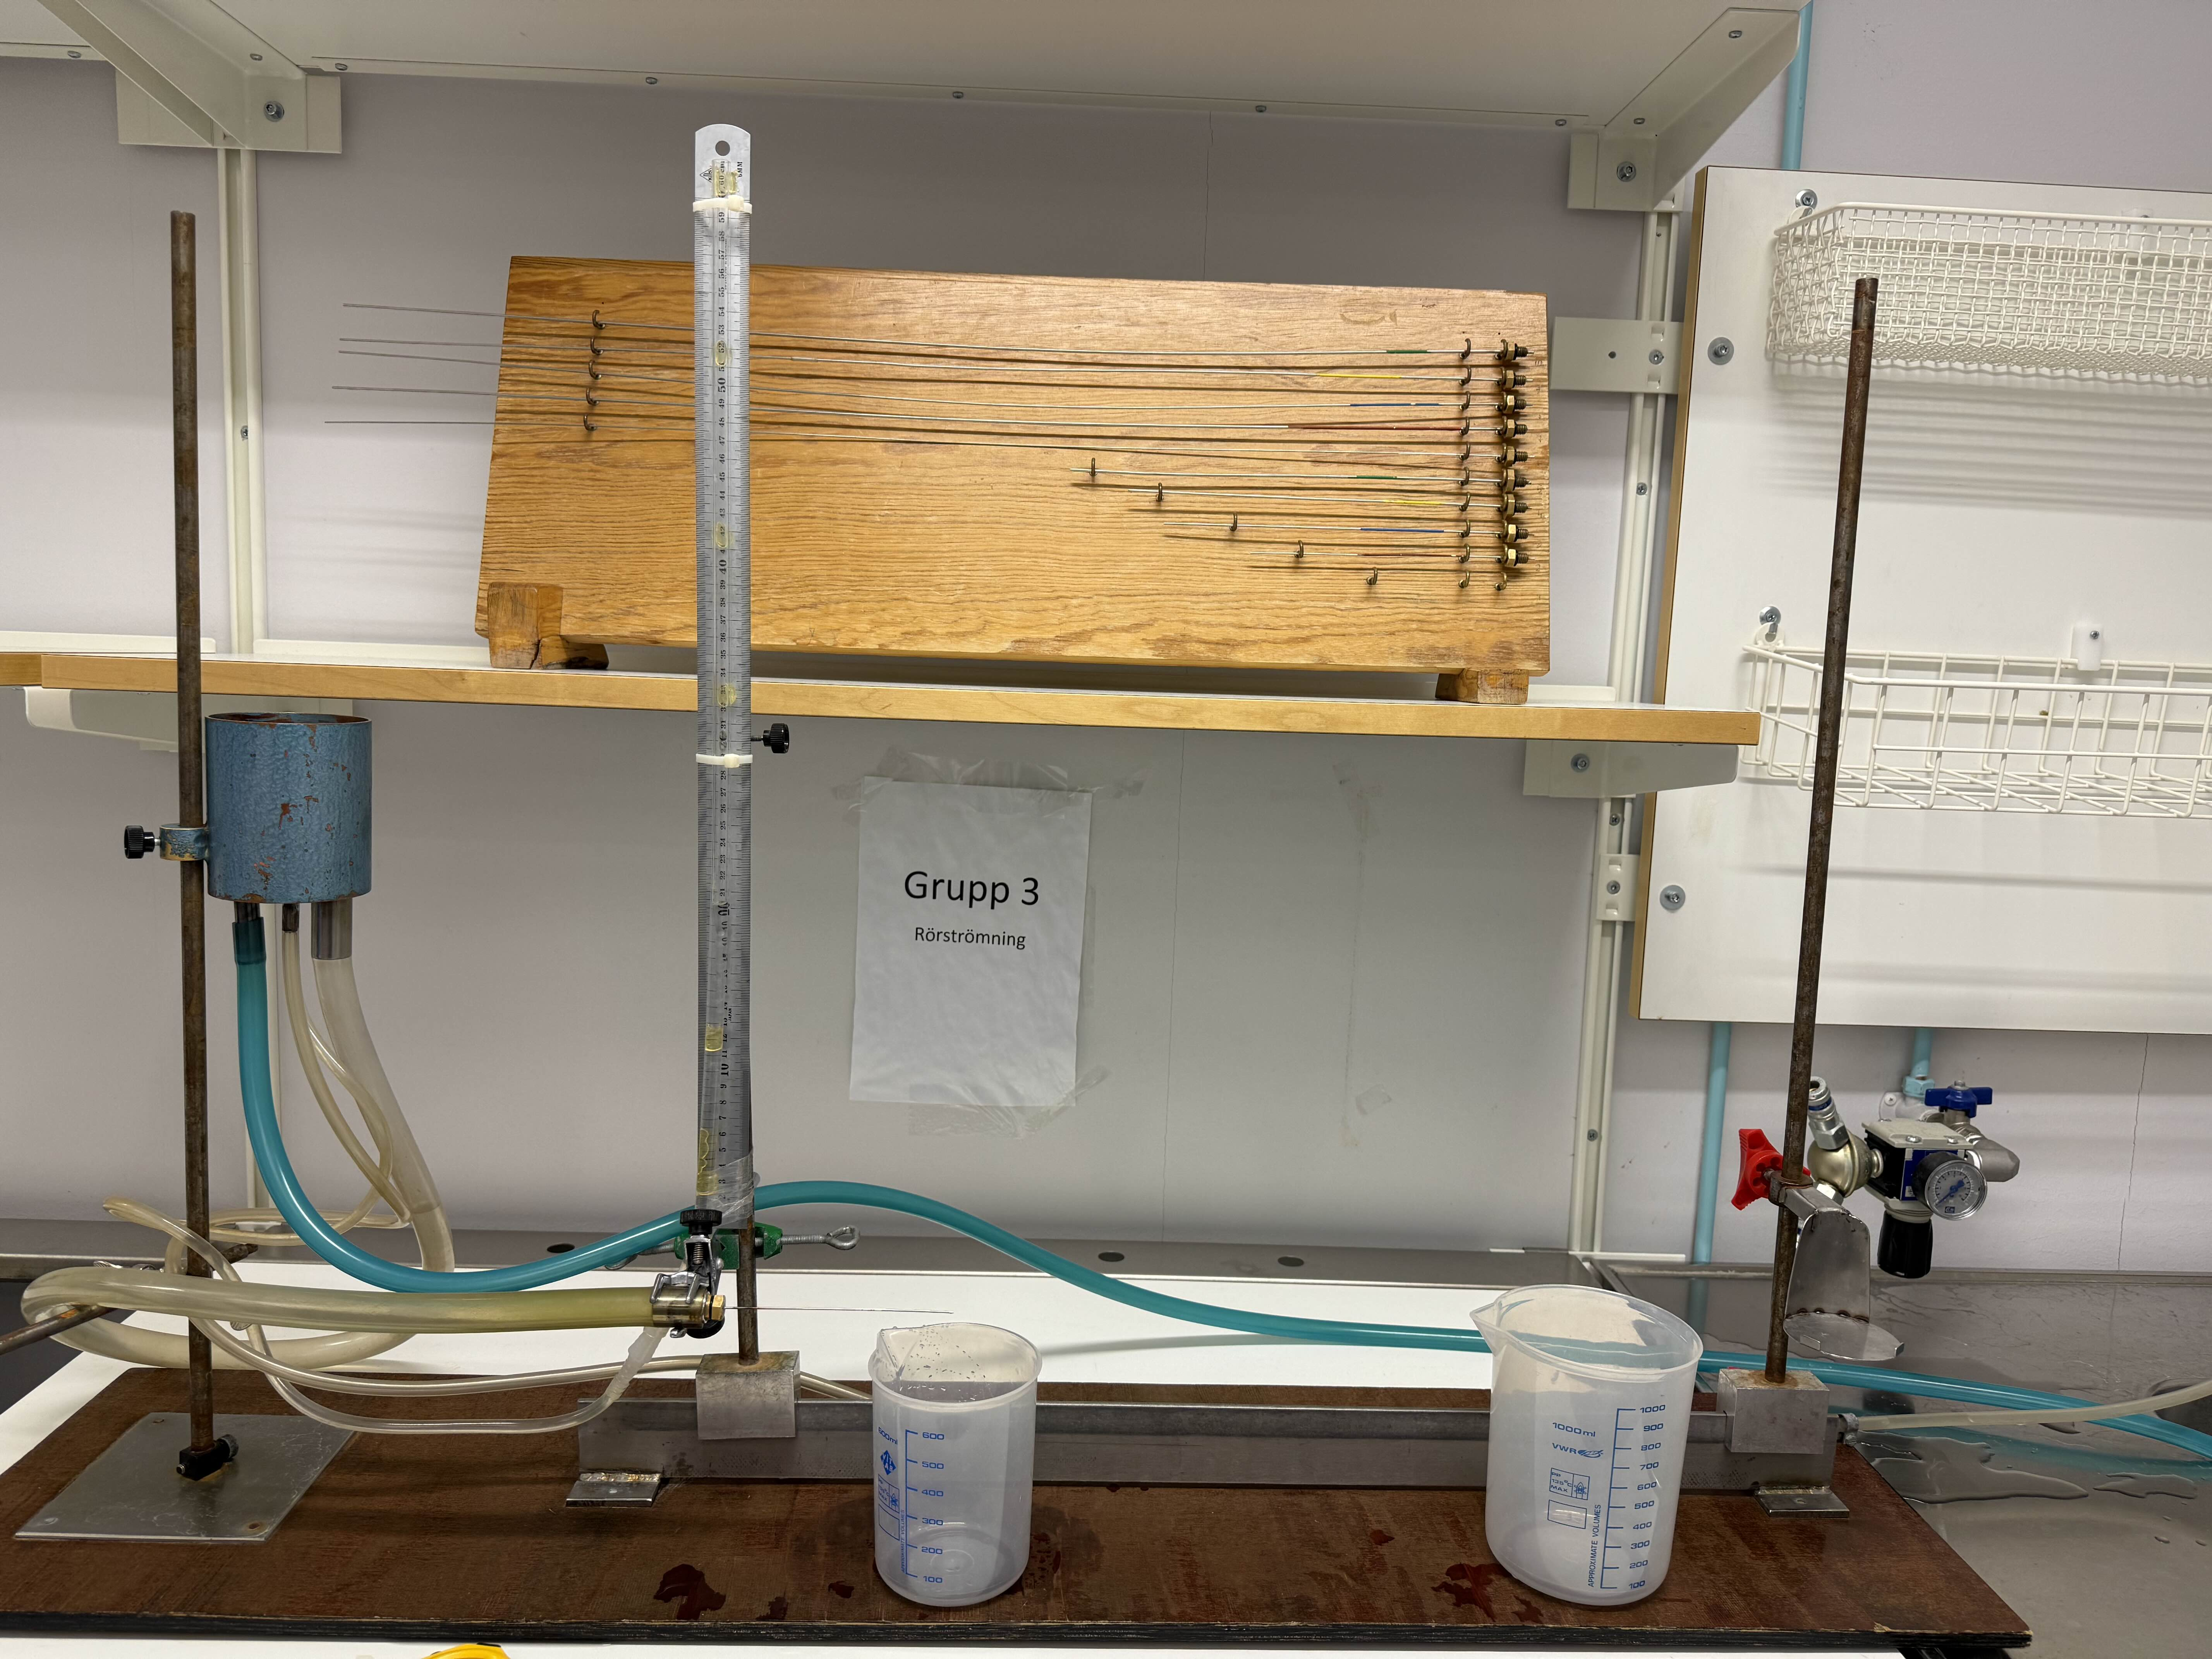
\includegraphics[width=0.5\textwidth]{Labb-yta.jpg}
    \caption{Experimentuppställning för flödesmätning.}
    \label{fig:experiment_setup}
\end{figure}
%
\noindent
Vattenflödet mättes genom att samla upp vatten under en bestämd tid i en vägd bägare. 
För varje mätning monterades ett specifikt rör beroende på vilken parameter som skulle 
undersökas. Efter att bägaren vägts, justerades vattenflödet till önskad nivå. 
Vattentrycket kontrollerades via glasrörets höjd när detta inte var den undersökta 
variabeln.
%
Mätningen påbörjades genom att placera bägaren under utloppet samtidigt som 
tidtagningen startades. Samtliga mätvärden dokumenterades i ett Excel-ark för 
senare analys. Experimentet undersökte tre variabler:
%
\begin{itemize}
    \item Rörradie
    \item Rörlängd
    \item Vattentryck
\end{itemize}
%
\begin{table}[ht]
    \centering
    \begin{tabular}{|l|c|c|}
        \hline
        \textbf{Storhet} & \textbf{Beteckning} & \textbf{Dimension} \\
        \hline
        Volymflöde & $Q$ & $L^3T^{-1}$ \\
        Rörlängd & $l$ & $L$ \\
        Rörradie & $r$ & $L$ \\
        Tid & $t$ & $T$ \\
        Volym & $V$ & $L^3$ \\
        Densitet* & $\rho$ & $ML^{-3}$ \\
        Tyngdacceleration* & $g$ & $LT^{-2}$ \\
        Viskositet* & $\mu$ & $ML^{-1}T^{-1}$ \\
        Höjd i glasrör (vattentryck) & $h$ & $L$ \\
        \hline
    \end{tabular}
    \caption{Experimentets variabler med tillhörande beteckningar och dimensioner. 
             Variabler markerade med * förblev konstanta under experimentet.}
\end{table}
%
\subsection{Material och mätprecision}
För vattenuppsamling användes två plastbägare för att minimera vattenspill. 
Slangarna bestod av mjukt gummi och plast med tillräcklig flexibilitet utan 
att påverka vattenflödet. Mätprecisionen för vattenmängden var 1 mm.
%
\section{Grafer och Resultat}
Vi kan få fram 3 exponenter genom att linjärisera data från experimenten, så vi
börjar med hur volymflödet beror på höjden: \\
\begin{center}
    \begin{tabular}{  c  c  c  c  }
        Höjd(m) & Flöde$(m^3/s)$ & ln(höjd) & ln(Q) \\ 
        \hline
        $0.15$ & $8.8750e-7$ & $-1.897120$ & $-13.93486$ \\
        $0.25$ & $1.3546e-6$ & $-1.386294$ & $-13.51205$ \\
        $0.35$ & $1.7158e-6$ & $-1.049822$ & $-13.27561$ \\
        $0.45$ & $2.1096e-6$ & $-0.798508$ & $-13.06903$ \\
        $0.55$ & $2.4738e-6$ & $-0.597837$ & $-12.90978$ \\
    \end{tabular}
\end{center}
Och om vi linjäriserar detta hittar vi exponenten \\
\begin{figure}[htbp]
    \centering
    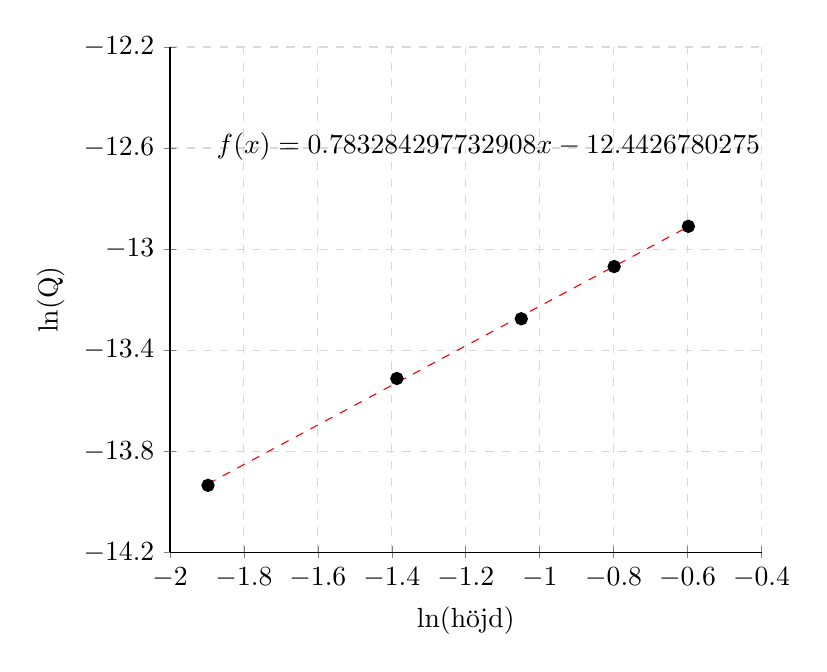
\begin{tikzpicture}
        \begin{axis}[
            xlabel={ln(\text{höjd})},
            ylabel={ln(Q)},
            xmin=-2, xmax=-0.4,
            ymin=-14.2, ymax=-12.2,
            width=0.75\textwidth,
            height=8cm,
            grid=major,
            grid style={dashed,gray!30},
            ytick={-14.2,-13.8,-13.4,-13,-12.6,-12.2},
            scaled y ticks=true,
            scaled x ticks=true,
            axis lines = left,
            axis line style={-},
        ]
            % Your data points here
            \addplot[thick,black,mark=*,only marks] coordinates {
                % Add your coordinates here
                (-1.89712, -13.9349)
                (-1.38629, -13.512)
                (-1.04982, -13.2756)
                (-0.79851, -13.069)
                (-0.59784, -12.9098)
            };
            \addplot[red,dashed] table[y={create col/linear regression={y=Y}}] {
                x       Y
                -1.89712 -13.9349
                -1.38629 -13.512
                -1.04982 -13.2756
                -0.79851 -13.069
                -0.59784 -12.9098
            };
                \node[anchor=north west] at (axis cs:-1.9,-12.5) {$f(x) =
                0.783284297732908 x - 12.4426780275189$};
        \end{axis}
    \end{tikzpicture}
    \label{fig:LNheight_flow}
\end{figure} \\
%
Sedan undersöker vi hur radien påverkar volymflödet, samt linjärisera \\
\begin{center}
    \begin{tabular}{  c  c  c  c  }
        Radie(m) & Flöde$(m^3/s)$ & ln(r) & ln(Q) \\ 
        \hline
        $0.000875$ & $1.2342e-6$ & $-7.041287$ & $-13.60511$ \\
        $0.000770$ & $7.3917e-7$ & $-7.169120$ & $-14.11774$ \\
        $0.000685$ & $4.9792e-7$ & $-7.286092$ & $-14.51283$ \\
        $0.000535$ & $1.8667e-7$ & $-7.533244$ & $-15.49394$ \\
        $0.000440$ & $8.9583e-8$ & $-7.728736$ & $-16.22810$ \\
    \end{tabular}
\end{center}
\begin{figure}[htbp]
    \centering
    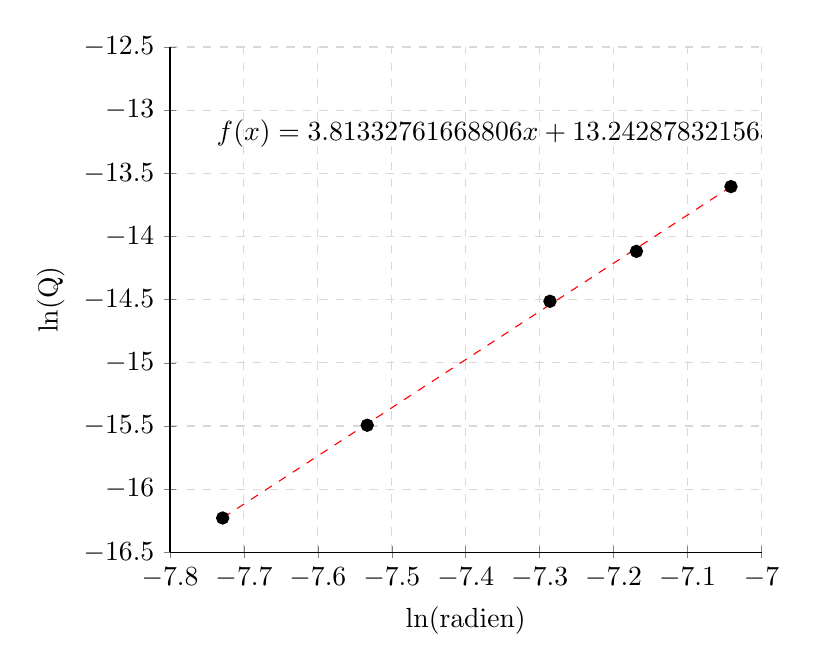
\begin{tikzpicture}
        \begin{axis}[
            xlabel={ln(\text{radien})},
            ylabel={ln(Q)},
            xmin=-7.8, xmax=-7,
            ymin=-16.5, ymax=-12.5,
            width=0.75\textwidth,
            height=8cm,
            grid=major,
            grid style={dashed,gray!30},
            ytick={-16.5,-16,-15.5,-15,-14.5,-14,-13.5,-13,-12.5},
            scaled y ticks=true,
            scaled x ticks=true,
            axis lines = left,
            axis line style={-},
        ]
            % Your data points here
            \addplot[thick,black,mark=*,only marks] coordinates {
                % Add your coordinates here
                (-7.04129, -13.6051)
                (-7.16912, -14.1177)
                (-7.28609, -14.5128)
                (-7.53324, -15.4939)
                (-7.72874, -16.2281)
            };
            \addplot[red,dashed] table[y={create col/linear regression={y=Y}}] {
                x       Y
                -7.04129 -13.6051
                -7.16912 -14.1177
                -7.28609 -14.5128
                -7.53324 -15.4939
                -7.72874 -16.2281
            };
            \node[anchor=north west] at (axis cs:-7.75,-13) {$f(x) =
            3.81332761668806x + 13.2428783215635$};
        \end{axis}
    \end{tikzpicture}
    \label{fig:LNRadius_flow}
\end{figure}
%
\newpage
Slutligen undersöker vi hur längden påverkar volymflödet, samt linjärisera \\
\begin{center}
    \begin{tabular}{  c  c  c  c  }
        Längd(m) & Flöde$(m^3/s)$ & ln(r) & ln(Q) \\ 
        \hline
        $0.347$ & $2.4738e-6$ & $-1.058430$ & $1.5853e+1$ \\
        $0.302$ & $1.7658e-6$ & $-1.197328$ & $1.6027e+1$ \\
        $0.277$ & $1.3025e-6$ & $-1.283738$ & $1.6191e+1$ \\
        $0.212$ & $5.6167e-7$ & $-1.551169$ & $1.6338e+1$ \\
        $0.150$ & $3.8375e-7$ & $-1.897120$ & $1.6740e+1$ \\
    \end{tabular}
\end{center}
\begin{figure}[htbp]
    \centering
    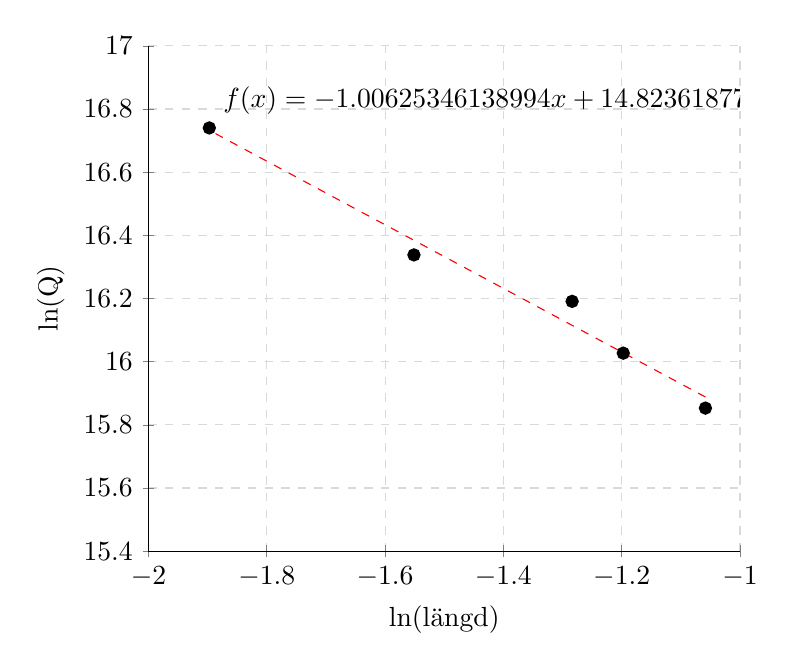
\begin{tikzpicture}
        \begin{axis}[
            xlabel={ln(\text{längd})},
            ylabel={ln(Q)},
            xmin=-2, xmax=-1,
            ymin=15.4, ymax=17,
            width=0.75\textwidth,
            height=8cm,
            grid=major,
            grid style={dashed,gray!30},
            ytick={15.4,15.6,15.8,16,16.2,16.4,16.6,16.8,17},
            scaled y ticks=true,
            scaled x ticks=true,
            axis lines = left,
            axis line style={-},
        ]
            % Your data points here
            \addplot[thick,black,mark=*,only marks] coordinates {
                % Add your coordinates here
                (-1.05843, 1.5853e+1)
                (-1.19733, 1.6027e+1)
                (-1.28374, 1.6191e+1)
                (-1.55117, 1.6338e+1)
                (-1.89712, 1.6740e+1)
            };
            \addplot[red,dashed] table[y={create col/linear regression={y=Y}}] {
                x       Y
                -1.05843 1.5853e+1
                -1.19733 1.6027e+1
                -1.28374 1.6191e+1
                -1.55117 1.6338e+1
                -1.89712 1.6740e+1
            };
            \node[anchor=north west] at (axis cs:-1.89,16.9) {$f(x) =
            -1.00625346138994x + 14.8236187761332$};
        \end{axis}
    \end{tikzpicture}
    \label{fig:LNLength_flow}
\end{figure}
%
\section{Dimensionsanalys av Volymflöde}
Det generella sambandet för volymflödet ges av:
\begin{equation}
    Q = C \cdot r^\alpha \cdot h^\beta \cdot l^\gamma \cdot \rho^\delta \cdot g^\epsilon \cdot \mu^\varepsilon
    \label{eq:general_flow}
\end{equation}
%
%där variablerna har följande dimensioner:
%\begin{itemize}
%    \item $Q$ är volymflödet [$\mathrm{L^3T^{-1}}$]
%    \item $r$ är rörets radie [$\mathrm{L}$]
%    \item $h$ är höjdskillnaden [$\mathrm{L}$]
%    \item $l$ är rörets längd [$\mathrm{L}$]
%    \item $\rho$ är vätskans densitet [$\mathrm{ML^{-3}}$]
%    \item $g$ är tyngdaccelerationen [$\mathrm{LT^{-2}}$]
%    \item $\mu$ är vätskans viskositet [$\mathrm{ML^{-1}T^{-1}}$]
%\end{itemize}
%
Genom att ta dimensionerna från volymflöde får vi
\begin{equation}
    [Q] = \mathrm{L^3T^{-1}M^0}
    \label{eq:dim_Q}
\end{equation}
%
\begin{equation}
    [Q] = [C] \cdot [d^\alpha] \cdot [h^\beta] \cdot [l^\gamma] \cdot [\rho^\delta] \cdot [g^\epsilon] \cdot [\mu^\varepsilon]
    \label{eq:dim_analysis}
\end{equation}
%
Från tidigare beräkningar har vi fått:
\begin{align}
    \alpha &= 4 \label{eq:alpha} \\
    \beta &= 1 \label{eq:beta} \\
    \gamma &= -1 \label{eq:gamma}
\end{align}
%
Genom att jämföra exponenter får vi:
\begin{align}
    \mathrm{L^3T^{-1}} &= \mathrm{L^{\alpha + \beta + \gamma}} \cdot 
    \mathrm{(ML^{-3})^\delta} \cdot \mathrm{(LT^{-2})^\epsilon} \cdot 
    \mathrm{(ML^{-1}T^{-1})^\varepsilon} \\
    \mathrm{L^3T^{-1}} &= \mathrm{M^{\delta + \varepsilon}} \cdot 
    \mathrm{L^{\alpha + \beta + \gamma - 3\delta + \epsilon - \varepsilon}} \cdot 
    \mathrm{T^{-2\epsilon - \varepsilon}}
\end{align}
%
Det resulterande ekvationssystemet blir:
\begin{align}
    \mathrm{M}&: \delta + \varepsilon = 0 \label{eq:M_balance} \\
    \mathrm{L}&: \alpha + \beta + \gamma - 3\delta + \epsilon - \varepsilon = 3 \label{eq:L_balance} \\
    \mathrm{T}&: -2\epsilon - \varepsilon = -1 \label{eq:T_balance}
\end{align}
%
Ur \cref{eq:M_balance} får vi:
\begin{equation}
    \epsilon = -\delta \label{eq:epsilon}
\end{equation}
%
Substitution i \cref{eq:L_balance} ger:
\begin{align}
    4 + 1 - 1 - 3\delta - \delta + \varepsilon &= 3 \\
    4 - 4\delta + \varepsilon &= 3 \\
    \varepsilon &= 2\delta - 1
\end{align}
%
från \cref{eq:T_balance}:
\begin{align}
    -1 &= -(-\delta) - 2(2\delta - 1) \\
    -1 &= \delta - 4\delta + 2 \\
    -3 &= -3\delta \\
    \delta &= 1
\end{align}
%
från det kan vi lösa \cref{eq:epsilon}
\begin{align}
    \epsilon = -\delta = -1
\end{align}
alltså får vi att exponenterna är
\begin{align}
    \delta &= 1 \\
    \epsilon &= -1 \\
    \varepsilon &= 2(1) - 1 = 1
\end{align}
%
\subsection*{Konstanten $C$}
För att bestämma konstanten $C$ använder vi oss av tidigare mätningar. Vi har mätt volymflödet för olika värden på $r$, $h$ och $l$. Genom att linjärisera dessa mätningar kan vi bestämma $C$ genom att använda linjens skärning med $y$-axeln.
\begin{figure}[H]
    \centering
    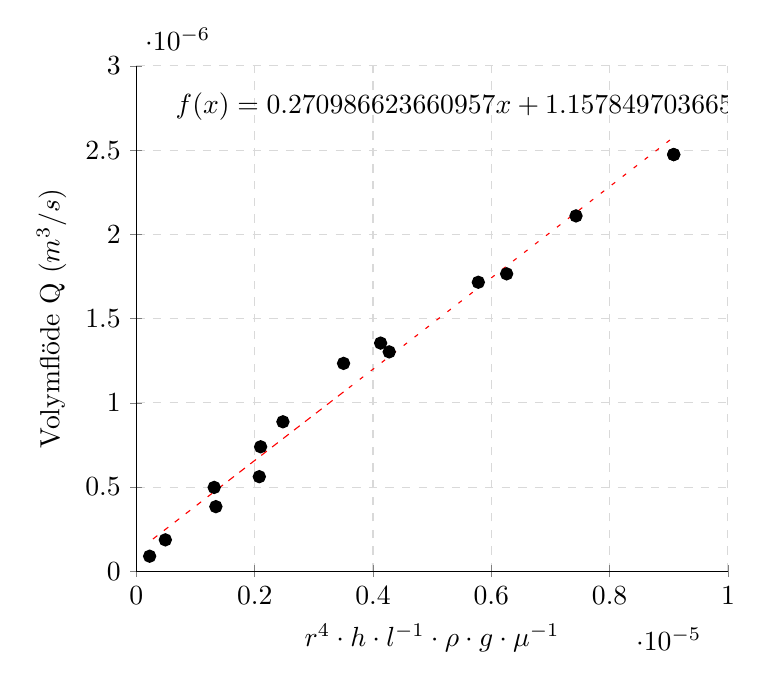
\begin{tikzpicture}
        \begin{axis}[
            ylabel={Volymflöde Q $(m^3/s)$},
            xlabel={$r^4 \cdot h \cdot l^{-1} \cdot \rho \cdot g \cdot \mu^{-1}$},
            xmin=0, xmax=1e-5,
            ymin=0, ymax=3e-6,
            width=0.75\textwidth,
            height=8cm,
            grid=major,
            grid style={dashed,gray!30},
            axis lines = left,
            axis line style={-},
        ]
            % Your data points here
            \addplot[thick,black,mark=*,only marks] coordinates {
                (0.0000035022, 0.0000012342)
                (0.0000021002, 0.00000073917)
                (0.0000013154, 0.00000049792)
                (0.00000048947, 0.00000018667)
                (0.00000022393, 0.000000089583)
                (0.0000024773, 0.0000008875)
                (0.0000041289, 0.0000013546)
                (0.0000057804, 0.0000017158)
                (0.0000074319, 0.0000021096)
                (0.0000090835, 0.0000024738)
                (0.0000090835, 0.0000024738)
                (0.000006259, 0.0000017658)
                (0.000004274, 0.0000013025)
                (0.0000020779, 0.00000056167)
                (0.0000013436, 0.00000038375)
            };
            \addplot[red,dashed,mark=none,dash pattern = on 1pt off 4pt,] table[y={create col/linear regression={y=Y}}] {
                x Y
                0.0000035022 0.0000012342
                0.0000021002 0.00000073917
                0.0000013154 0.00000049792
                0.00000048947 0.00000018667
                0.00000022393 0.000000089583
                0.0000024773 0.0000008875
                0.0000041289 0.0000013546
                0.0000057804 0.0000017158
                0.0000074319 0.0000021096
                0.0000090835 0.0000024738
                0.000006259 0.0000017658
                0.000004274 0.0000013025
                0.0000020779 0.00000056167
                0.0000013436 0.00000038375
            };
            \node[anchor=north west] at (axis cs:0.0000005,0.0000029) {$f(x) =
            0.270986623660957x +1.15784970366569e-7$};
        \end{axis}
    \end{tikzpicture}
    \label{fig:constant}
\end{figure}
funktionen ger oss konstanten:
\begin{align}
    C = 0.270986623660957 \approx 0.271.
\end{align}
\section{Diskussion och slutsats}
%
I denna labboration undersöktes hur volymflödet av vatten genom horisontella, tunna rör påverkas av parametrar såsom fallhöjd, rörets längd och rörets radie. Genom dimensionsanalys och linjarisering kunde en funktion härledas som på ett övergripande plan stämde överens med förväntade samband. Resultaten indikerar att volymflödet ökar med ökande fallhöjd. Vidare observerades en ökning av volymflödet då rörets längd minskar samt att rörets radie påverkar genom att större radie medger ett större tvärsnitt för strömningen, vilket ökar volymflödet.
%
\subsection{Felkällor}
Ett antal felkällor kunde identifieras under experimentets gång. Den mänskliga faktorn vid tidtagning utgjorde en felkälla, då samtliga mätningar byggde på att en bägare placerades under röret i exakt 60 sekunder. Även små avvikelser i tidtagningen påverkar noggrannheten i den uppmätta volymen. En mer tillförlitlig metod vore att använda elektroniska flödesmätare eller automatiserade ventiler som stänger flödet efter en förutbestämd tid.
%
En annan utmaning var att säkerställa att röret låg exakt horisontellt. Små avvikelser i rörets lutning kan förändra det effektiva tryckfall som driver flödet. Rörens egenvikt ledde till svag nedböjning, framför allt hos längre rör, vilket ytterligare komplicerade försök att uppnå full horisontalitet. Ett mer robust stativ med möjlighet till finjustering, alternativt användning av precisionsinstrument såsom vattenpass eller laserbaserade mätinstrument, skulle minska denna felkälla.
%
Ytterligare felkälla var rörets radie, som enligt instruktionerna kunde avvika inom ett intervall av $\pm 0,04$--$0,07$ mm. 
Även mätfel i höjdskillnaden hos vattenpelaren introducerar osäkerheter i det tryck som driver flödet. Noggrannare mätmetoder, exempelvis optiska sensorer eller mer avancerad lasermätning av rördimensioner och vattennivå, skulle ge säkrare resultat.
%
Vattnets temperatur mättes inte systematiskt, vilket kan ha påverkat både densitet och viskositet. Variationer i dessa kan förändra flödesegenskaperna. Att upprätthålla en konstant och känd temperatur, eller att kompensera för temperaturvariationer genom kontinuerlig mätning, skulle ge mer tillförlitliga resultat.
%
Slutligen försummades friktionsförluster i rörsystemet samt turbulent flöde som potentiellt kan påverka mätresultaten.
\subsection{Slutsats}
Trots nämnda felkällor kunde experimentet ge en formel som beskriver volymflödet i tunna, horisontella rör, vilket blev:
\[
Q = 0.271 \cdot r^4 \cdot h \cdot l^{-1} \cdot \rho \cdot g \cdot \mu^{-1}.
\]
Genom förbättringar i mätmetodik, mer precis utrustning samt noggrannare kontroll av fysiska parametrar som temperatur, lutning och rördimensioner, kan tillförlitligheten hos resultatet öka. 
%
\end{document}
